%%=============================================================================
%% Conclusie
%%=============================================================================

\chapter{Discussion}
\label{ch:conclusie}

Quantum computing will most definitely become one of the great buzzwords of the next decade. With the release of \textcite{Google2019} around their interpretation of 'Quantum supremacy', the whole field was catapulted to the forefront of research. All big players in Quantum research have been given a tremendous spotlight for the future of profitable quantum computing. And this is precisely why we need to make the concept more approachable for anybody interested.

\subsection{Quantum computing for now}

Firstly, after thorough research, a couple of interesting conclusions can be drawn. Beginning with one of the most important ones, Quantum computing is here to stay. The technology has given too much promise in too many sectors that have a strong financial backbone. At this point it is important to understand that the world around us that is visible with the naked eye is completely homogeneous with the 'quantum world', meaning that all research to exploring our world around us, can only prove to be profitable in the future.

Secondly returning to the more concrete conclusions of this paper. While executing this specific version of Grover's algorithm, there was a clear trend visible between the theory and the practical example that does show there are some growing pains that come with the expansion of our quantum devices.
Yes, the theory can be fully implemented at this point to visualise its results when we would work in the most perfect of environments like a simulator. But this perfect environment simply does not exist. Meaning that we will have to be creative to reach this edge of perfect conditions to get to a point that these simulated algorithms can become reliable and profitable towards the future. There are two ways of trying to fix the issue of quantum decoherence. Firstly we could create devices that are not influenced by any internal/ external interferences. They could provide a stable platform for algorithms like Shor's encryption breaking algorithm \textcite{gidney2019factor}. The other option would be to account for these interferences to happen anyway and try and compensate them in a software way, much in the same way a computer does error correction for downloaded files. The latter seems to be the more reasonable option where we are already trying to implement these quantum error correction in to provide better results \autocite{Cory1998}. For now there is no clear technique behind the whole principle except to play around with the length that a qubit needs to stay in its elevated $\ket{1}$ state and the length of the circuit as a whole

But this can all be tried out. Because at the moment we are able to extensively experiment with real or simulated quantum devices. There is a multitude of platforms available, most of them are open-source and free to contribute to them as you want to expand their feature-set. Frameworks like Qiskit allow users to design quantum circuits and test them using their built in simulators, which are easy to pick up but hard to master. As of now IBMQ is the only service that allows you to push up your circuits to really test them on a real device owned and managed by IBM. By granting people the privilege to experiment around with the real devices and notice the shortcomings through raw data results, really shows off how dedicated the whole community of computer science is on pushing this technology to the forefront.


\subsection{Quantum computing and its myths}

As shown in the experiment, QC will not change our entire world in the next year in any drastic manner. So theories that quantum computing could break our entire encryption standard in a matter of years seem absurd once you look at the real executions of these needed algorithms on real quantum devices.
Nevertheless we do want to work proactively to have solutions ready-to-go once these machines do become powerful enough to brute force the RSA-encryption by finding the factors of the prime numbers that represent the private keys of encrypted files.
Some researchers also believe that quantum decoherence will prove to be an unpassable obstacle the more qubits we start adding to the systems. This obstacle is the fact that adding more qubits to a system will always increase the internal interference exponentially and thus generate too much decoherence. This indeed is a major hurdle that needs to be overcome to make quantum computing the new standard for solving really hard to solve problems in the computer science community.

\subsection{Quantum computing as an addition}

The one thing we should take away from the dawn of quantum computing the following decade, is that quantum computing is not the one solution for every single issue in computing. It has its advantages and disadvantages just like classical computing. We should strive to make these two technologies as complementary as possible so that they can cancel out each others disadvantages and amplify their advantages. 

With this work, we have tried to inspire people to learn more about the subject of quantum computing and to hopefully entice them into writing their own 'Hello-world-Applications' on any of the freely available frameworks. For the actual executions and setup of the used experiments, we refer to appendix A.

\subsection{Future works}

The potential powerhouse of a mainframe device and a quantum computer can still prove to be advantageous in future works. If IBM keeps up with doubling its pace of releasing quantum computational resources into the world each year, there may be a chance that mainframes and QC prove to be viable in the near future. Also quantum error correction needs to evolve to an acceptable percentage to where we could start thinking about implementing QC machine learning algorithms in our mainframes or even the speeding up the database structures in the devices by using algorithms like Grover's. But for now QC and mainframe are not able to cooperate in an useful manner to add more business value. 

It is useful to explore these options upfront so that we know when the time comes to expand QC towards the mainframe we have a clear scope to all the potential applications of these two devices.


\begin{figure}[h]
	\centering
	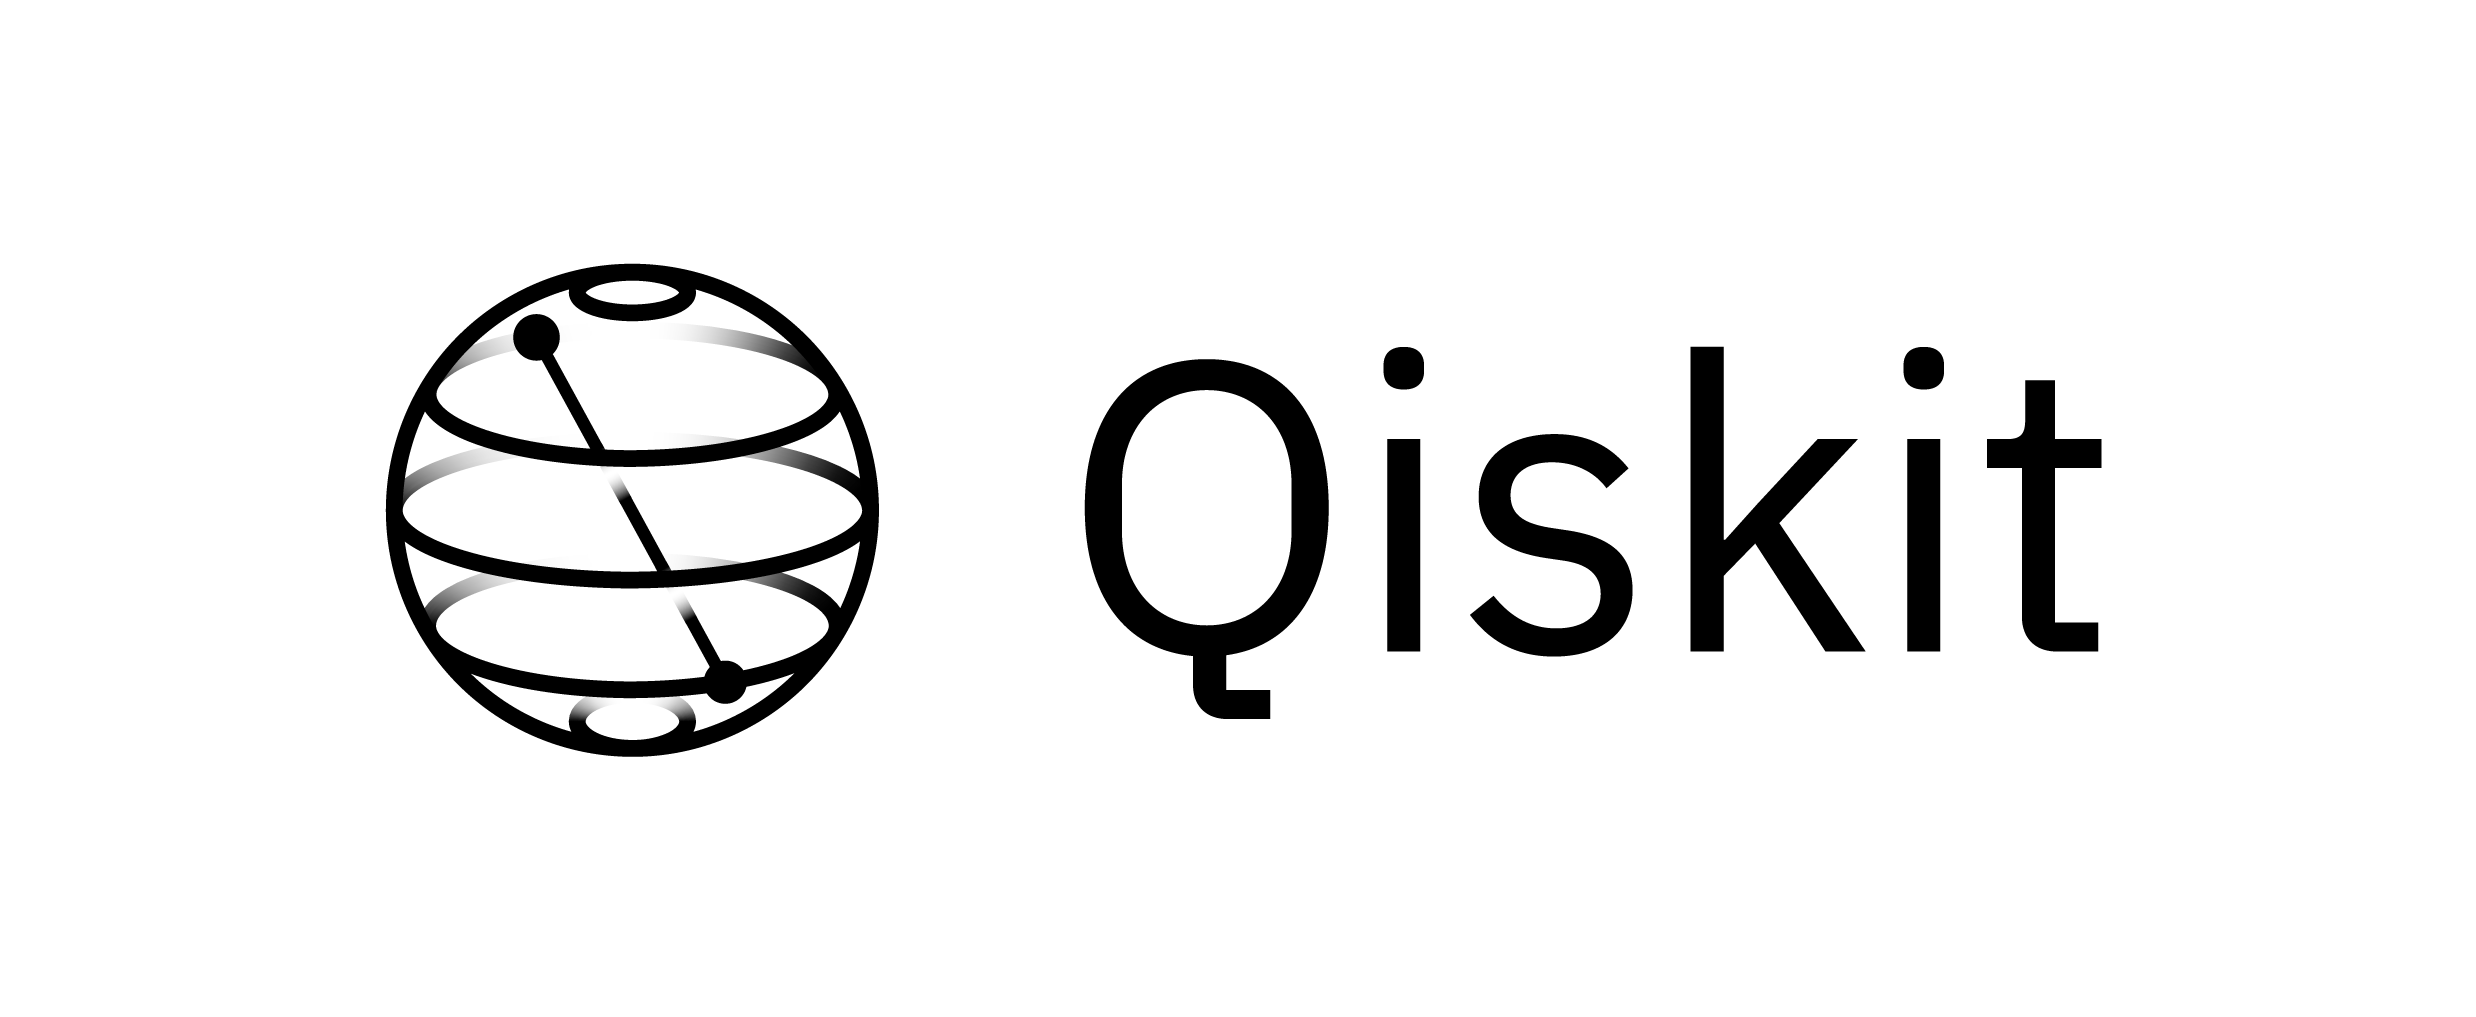
\includegraphics[scale = 0.75]{../Demonstration/img/qiskit_logo.PNG}
	\caption{The platform we used for executing the 3-SAT algorithm on a real quantum device. © Copyright 2020, Qiskit Development Team Last updated on 2020/05/14.}
\end{figure}


